\hyperref[acro:VISOR]{VISOR}\textsuperscript{\textregistered} software is not officially supported by the \hyperref[acro:KR]{KR1410} and there is no direct integration of the \hyperref[acro:VISOR]{VISOR}\textsuperscript{\textregistered} camera available.
However, Kassow robots provides support to build own software through \hyperref[acro:CBun]{CBun} development.
The \hyperref[acro:CBun]{CBun} (Capability Bundle) represents a modular framework within the \hyperref[acro:KR]{KR} software system,
which encapsulates functionalities and provides the
access to its predefined \hyperref[acro:API]{API}.


\begin{figure}[h]
    \centering
    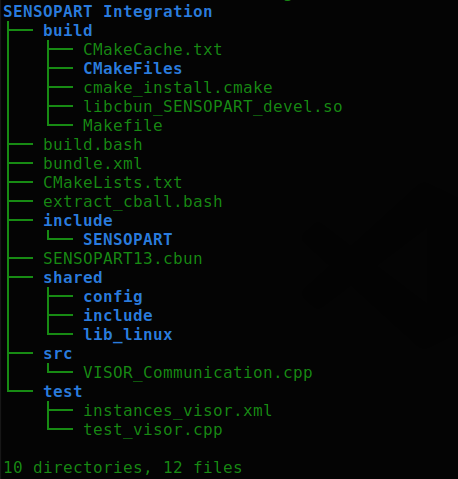
\includegraphics[width=0.5\textwidth]{figures/sensopart-development.png}
    \caption{\hyperref[acro:CBun]{CBun} Project Setup for SENSOPART Integration in KR}
    \label{fig:sensopart-development}
\end{figure}


The \hyperref[acro:CBun]{CBun} SDK is the Software Development Kit that provides all essential tools
for \hyperref[acro:CBun]{CBun} development. The project setup is created in a Visual Studio Code container
running on Ubuntu 18.04 with a special set of software packages. \cite{Cbun}
The header files are located in \textbf{include} directory and C++ source file \textit{i.e.}     \textit{VISOR\_Communication.cpp}
are placed in \textbf{src} directory.
Upon building the project, a \textit{SENSOPART.cbun} file is generated as shown in \ref{fig:sensopart-development}
It is then installed in the teach pendant using a \hyperref[acro:USB]{USB}.

\begin{figure}[h]
    \centering
    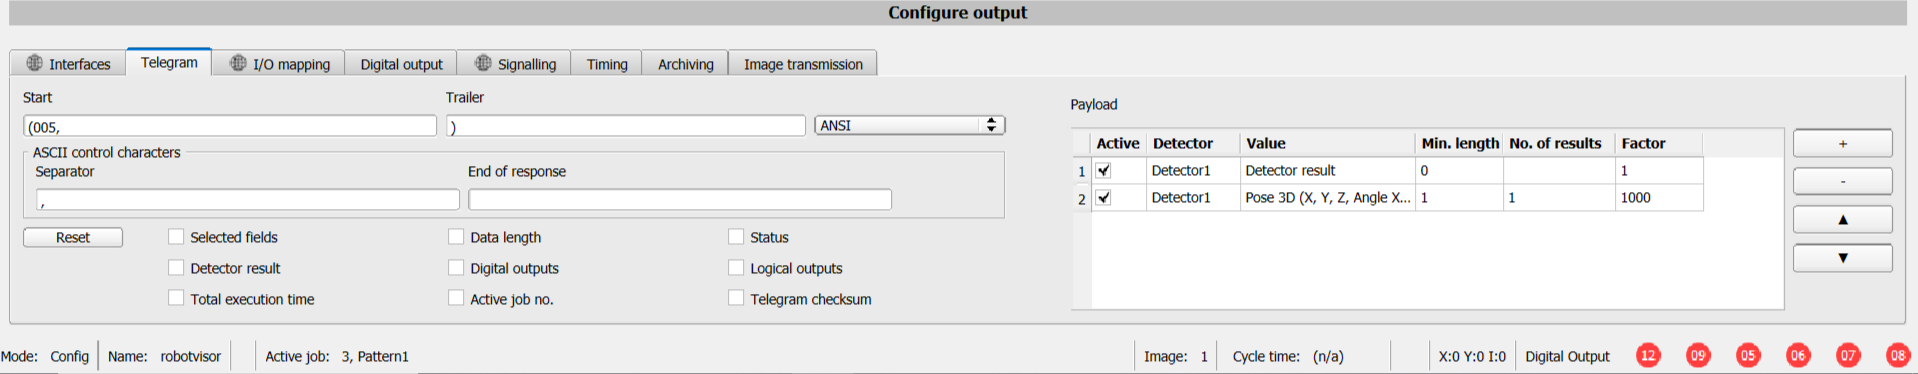
\includegraphics[width=1\textwidth]{figures/telegram-output.png}
    \caption{\hyperref[acro:VISOR]{VISOR}\textsuperscript{\textregistered} Communication to KR1410 using Telegram}
    \label{fig:visor-communication}
\end{figure}

\hyperref[acro:CBun]{CBun} device is one of the \hyperref[acro:CBun]{CBun} elements. \hyperref[acro:CBun]{CBun} Device concept allows to wrapping handling code of physical device like \hyperref[acro:VISOR]{VISOR}\textsuperscript{\textregistered} vision sensor into the \hyperref[acro:CBun]{CBun} and hide it from the end user. This allows the user to simply control and monitor devices without the need to implement the communication and logic. \cite{cbun-device}

\hyperref[acro:VISOR]{VISOR}\textsuperscript{\textregistered} camera is powered from the TPSU02 on the KR1410 tool-IO.
A \hyperref[acro:CBun]{CBun} device named \textbf{VISOR} from \hyperref[acro:CBun]{CBun} development is created which has methods for
controlling the functionalities of camera like changing job, getting object pose by triggering camera and performing calibration. Through this
device, the \hyperref[acro:KR]{KR} communicates with the \hyperref[acro:VISOR]{VISOR}\textsuperscript{\textregistered} over telegram. Figure \ref{fig:visor-communication} shows the setup of telegram with the correct start, trailer and separator characters, and also the transfer of data which only happens in the format of one integer and one pose value. The integer value is used for now to determine if the camera has detected the object while the pose value is used to send the pose of the detected object. Integer value of 1 means the camera has detected the object and 0 means not detected.


